\begin{lemma}
The points of intersection of \textbf{Line} $L:\vec{x}=\vec{q}+\mu\vec{m}$ with the conic 
\begin{align}
\vec{x^T}\vec{V}\vec{x}+2\vec{u^T}\vec{x}+f=0
\end{align}
are given by:
\begin{align}
\vec{x}_i = \vec{q}+\mu_i\vec{m}
\end{align}
%
where,
\begin{multline}
\mu_i = \frac{1}
{
\vec{m}^T\vec{V}\vec{m}
}
\lbrak{-\vec{m}^T\brak{\vec{V}\vec{q}+\vec{u}}}
\\
\pm
{\small
\rbrak{\sqrt{
\sbrak{
\vec{m}^T\brak{\vec{V}\vec{q}+\vec{u}}
}^2
-
\brak
{
\vec{q}^T\vec{V}\vec{q} + 2\vec{u}^T\vec{q} +f
}
\brak{\vec{m}^T\vec{V}\vec{m}}
}
}
}\label{sep/2/77/quad}
\end{multline}
\end{lemma}
For the given conic, the matrix parameters  are
\begin{align}
\vec{V}=\myvec{1&0\\0&0},\vec{u}=\myvec{0\\-2},f=0 \label{sep/2/77/quadform/2/105/eq:v}
\end{align}
with eigen parameters 
\begin{align}
\lambda_1 &= 0 , \lambda_2 = 1
\\
\vec{p_1} &= \myvec{0 \\ 1},
\vec{p_2} = \myvec{1 \\ 0}
\end{align}
The vertex of the parabola can be expressed as
\begin{align} \myvec{\vec{u^T}+\eta\vec{p_1^T}\\\vec{V} }\vec{c} &= \myvec{\vec{-f}\\\eta \vec{p_1} -\vec{u}}
\end{align}
where, 
\begin{align}\eta = \vec{u^T}\vec{p_1} = -2
\\
\implies\myvec{0 & -2\\1 & 0 \\0 & 0} \vec{c}&= \myvec{0\\0\\0}
\end{align}
or
\begin{align}
   \vec{c} &= \myvec{0 \\ 0}
\end{align}
From  \eqref{sep/2/77/quad},
\begin{align}
\mu_1 &= 4+2\sqrt{3}, \mu_2 =4-2\sqrt{3}
\end{align}
The given line is
\begin{align} 
\myvec{1&-1}\vec{x}&=-2
\end{align}
 In parametric form, the given  line can be written as:
\begin{align} 
L: \vec{x}&=\vec{q}+\mu\vec{m}
\\
\implies \vec{x}&=\myvec{-2\\0}+\mu\myvec{1\\1} \label{sep/2/77/quadform/2/105/eq:q}
\end{align}
Substituting $\mu_1$ and $\mu_2$ in \eqref{sep/2/77/quadform/2/105/eq:q},the points of intersection
\begin{align}
 \vec{K}= \myvec{2+2\sqrt{3}\\4+2\sqrt{3}},  
\vec{L}&= \myvec{2-2\sqrt{3}\\4-2\sqrt{3}}
\end{align}

\begin{enumerate}
  \item Thus, from Fig. \ref{sep/2/77/Plot of the Parabola and line} the area enclosed by parabola and line can be given as
\begin{align}
   A&= \text{Area under line} - \text{Area under parabola}
     \\
   A&= Ar(KLMNK)-Ar(KCLMCNK)
    \\
    A&= A_1 -A_2 \label{sep/2/77/eqAREA}
    \end{align}
\item Area under the line y=x+2 i.e, $A_1$-
\begin{align}
  A_1&= \int_{2-2\sqrt{3}}^{2+2\sqrt{3}} y dx
    \\
   &= \int_{2-2\sqrt{3}}^{2+2\sqrt{3}} \brak{x+2} dx\\
   &= \int_{2-2\sqrt{3}}^{2+2\sqrt{3}}x dx+\int_{2-2\sqrt{3}}^{2+2\sqrt{3}}2 dx\\
    &= \frac{1}{2}\brak{(2+2\sqrt{3})^2-(2-2\sqrt{3})^2} +2\brak{4\sqrt{3}}
    \\
    &=16\sqrt{3} \text{ units} \label{sep/2/77/eqB}
\end{align}
\item Area under the parabola that is $A_2$-
\begin{align}
    A_2&= \int_{2-2\sqrt{3}}^{2+2\sqrt{3}} y dx
    \\
    &= \int_{2-2\sqrt{3}}^{2+2\sqrt{3}} \frac{1}{4} x^2 dx
    \\
   &= \frac{1}{12} \int_{2-2\sqrt{3}}^{2+2\sqrt{3}} x^3 dx
    \\
    &= \frac{1}{12} \brak{(2+2\sqrt{3})^3-\brak{2-2\sqrt{3}}^3}
    \\
    &= 8\sqrt{3} \text{ units} \label{sep/2/77/eqC}
\end{align}
\item Putting \eqref{sep/2/77/eqB} and \eqref{sep/2/77/eqC} in \eqref{sep/2/77/eqAREA} we get required area A as:
\begin{align}
 A &= A_1 -A_2 
 \\
 A &= 8\sqrt{3} \text{ units}
\end{align}
%
\end{enumerate}
\begin{figure}[ht]
\centering
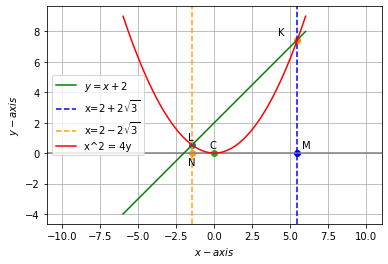
\includegraphics[width=\columnwidth]{solutions/sep/2/77/figures/parabola.png}
\caption{Plot of the parabola and line}
\label{sep/2/77/Plot of the Parabola and line}
\end{figure}

